% !TEX root = main.tex

\documentclass{beamer}
\usepackage{listings}
\usepackage{booktabs}
\usepackage{bookmark}
\usepackage{makecell}
\usepackage{url}
\usepackage{multirow}
\usepackage{graphicx}
\usepackage{hyperref}

\usepackage{beamerthemesplit}
\usetheme{Frankfurt}

\lstdefinestyle{latexStyle}{
    language=[LaTeX]{TeX},
    belowcaptionskip=1\baselineskip,
    breaklines=true,
    frame=none,
    numbers=none, 
    basicstyle=\footnotesize\ttfamily,
    keywordstyle=\bfseries\color{green!40!black},
    commentstyle=\itshape\color{purple!40!black},
    identifierstyle=\color{blue},
    backgroundcolor=\color{gray!10!white},
}
\lstset{style=latexStyle}

\title{Moogle!}
\institute{Facultad de Matemática y Computación\\Universidad de la Habana}
\author{Luis Alejandro Arteaga Morales}
\date{Julio, 2023}

\begin{document}
\maketitle

\section{Introducción}\label{sec:intro}

\begin{frame}{Introducción}
    Moogle! es un buscador simple que le permite al usuario encontrar en una base de documentos los más relevantes para un input dado.
    \begin{center}        
        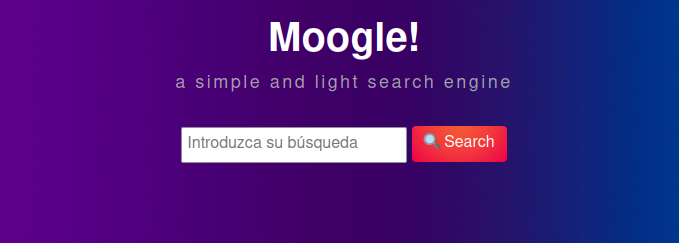
\includegraphics[height=100pt]{moogle.png}
    \end{center}
\end{frame}

\section{Buscador}\label{sec:how}

\subsection{¿Cómo buscar?}
\begin{frame}{¿Cómo buscar?}
    En la barra de búsqueda escriba las palabras que quiere buscar (note que puede buscar no solo palabras, sino una frase en sí) y presione el botón Search
\end{frame}

\subsection{¿Qué muestra?}
\begin{frame}{¿Qué me mostrará el buscador una vez realizada mi consulta?}
    Se le mostrará una lista de documentos que contengan las palabras que aparecen en su búsqueda. Si escribe una consulta vacía el buscador se lo informará. Se mostrarán primero los documentos que contienen palabras más raras (aparecen en la consulta pero aparecen en menos documentos). Las palabras que son demasiado comunes (aparecen en todos los documentos) no serán relevantes y por tanto ignoradas por la búsqueda
\end{frame}

\section{Funcionalidades Opcionales}
\begin{frame}{Funcionalidades Opcionales 1/2}
    \begin{itemize}
        \item Sugerencias: Si no se encuentra ningún resultado para su búsqueda se mostrará una sugerencia de lo que debería escribir en su consulta para tener resultados. Esta sugerencia está basada en palabras ya contenidas en los textos que sean lo más parecidas a la consulta inicial. Lucirá de la manera siguiente:
        ¿Quisite decir "sugerencia"?
        \item !palabra Los documentos que contengan las palabras que tengan un signo ! delante, no serán sugeridos
        \item \textasciicircum palabra Solo podrán ser sugeridos documentos que contengan las palabras que tengan un signo \textasciicircum  delante
        \item *palabra Cualquier cantidad de * delante de una palabra aumenta la relevancia de esta para la búsqueda
    \end{itemize}
\end{frame}

\begin{frame}{Funcionalidades Opcionales 2/2}
    \begin{itemize}
        \item palabra1 \textasciitilde  palabra2 Para dos o más palabras unidas por \textasciitilde, entre más cerca estén esas palabras en un documento más relevante será este
    \end{itemize}

    Nota:
    Para usar los operadores en una consulta es importante respetar las siguientes reglas: Los operadores ! \textasciicircum * deben estar pegados a la palabra de lo contrario la búsqueda se realizará pero estos no tendrán efecto No deben aparecer operadores intercalados. Por ejemplo: !\textasciicircum o *\textasciicircum Todos los operadores, menos \textasciitilde pueden repetirse. Si lo repetimos, este será ignorado
    \\
    No se recomienda usar símbolos extraños que no sean considerados letras o números en la búsqueda, puede que no obtenga los resultados esperados
\end{frame}

\section{Repositorio}
\begin{frame}{Repositorio del proyecto}
    Repositorio:
    \begin{itemize}
        \item \href{https://github.com/Sekai02/moogle-1}{https://github.com/Sekai02/moogle-1}
    \end{itemize}
\end{frame}

\end{document}